\chapter{Perancangan}
\label{chap:perancangan}
Pada bab ini akan dijelaskan mengenai perancangan aplikasi yang akan dibangun meliputi perancangan kelas, \textit{routes}, \textit{controllers}, \textit{models}, \textit{folder} ``public/'', dan perancangan antarmuka.

\section{Perancangan Kelas}
\label{sec:diagramkelas}
Seperti yang telah dijelaskan pada bab analisis, bahwa untuk memodelkan KIRI \textit{Dashboard} dalam Play Framework membutuhkan \textit{routes}, \textit{controllers}, \textit{models}, dan \textit{folder} ``public/''. Berdasarkan hasil pengembangan diagram kelas tahap analisis (Gambar \ref{fig:3_classdiagram_kasar}), dibuatlah diagram kelas rinci untuk memenuhi kebutuhan dalam membangun aplikasi sistem usulan (Gambar \ref{fig:4_classdiagramatribut} dan Gambar \ref{fig:4_classdiagramrelasi}). Deskripsi kelas beserta fungsi dari diagram kelas akan dijelaskan pada subbab selanjutnya.

\begin{figure}[htbp]
	\centering
		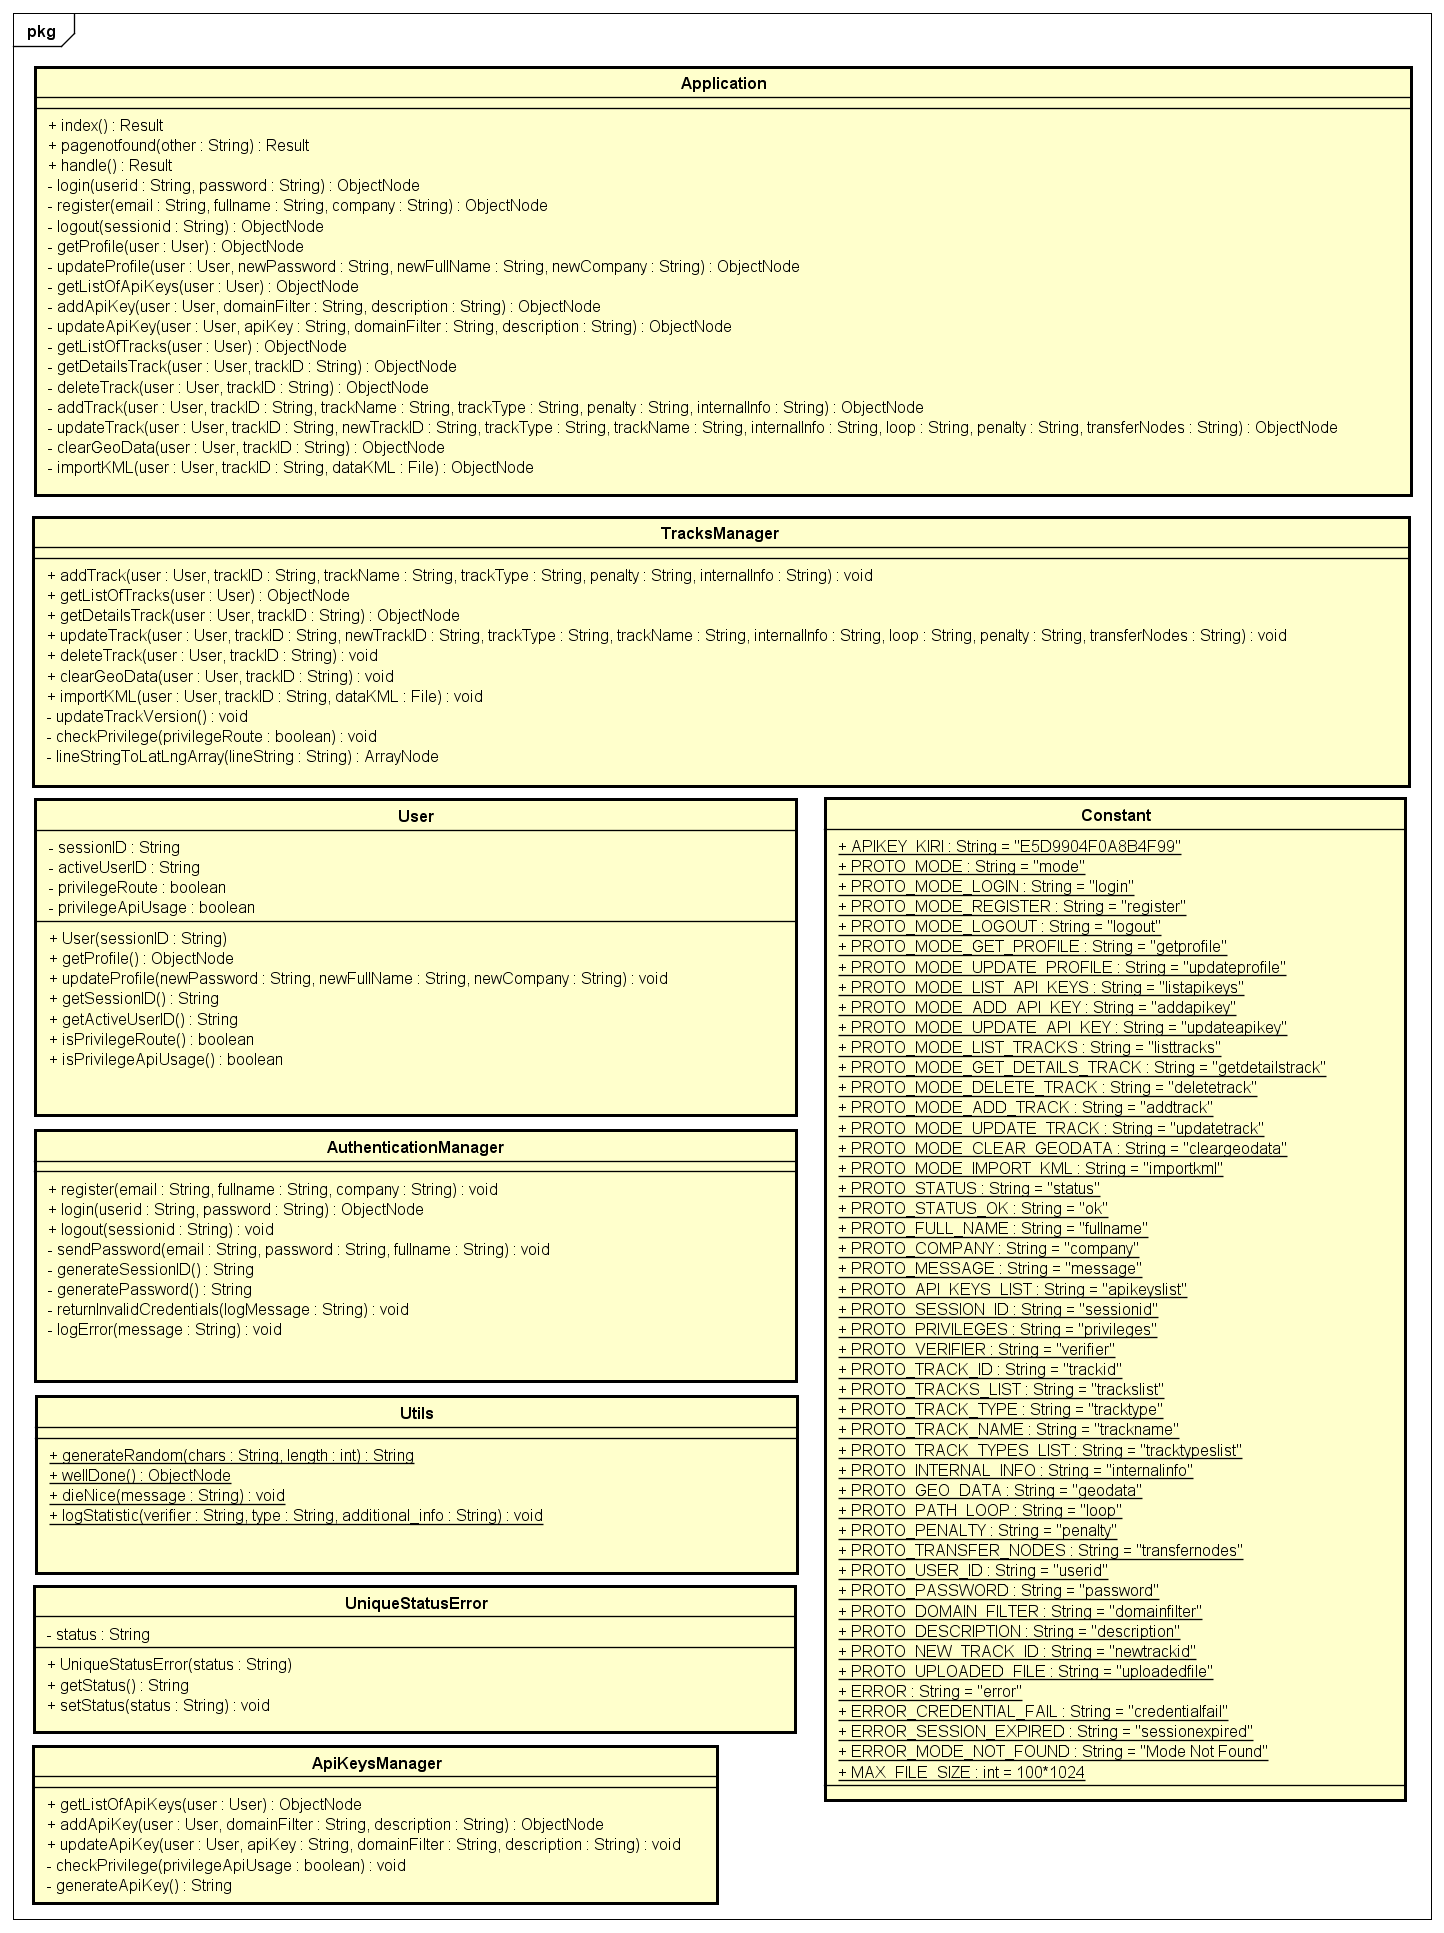
\includegraphics[scale=0.45]{Gambar/4_classdiagram_atribut.png}
	\caption{Kelas diagram rinci KIRI \textit{Dashboard server side} (atribut dan \textit{method})}
	\label{fig:4_classdiagramatribut}
\end{figure}

\begin{figure}[htbp]
	\centering
		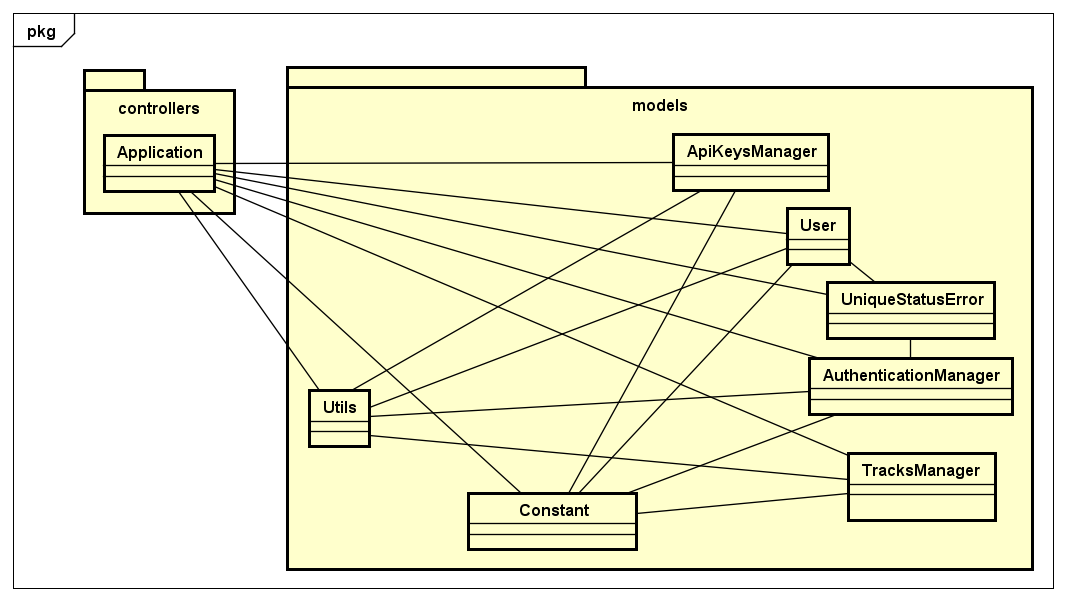
\includegraphics[scale=0.55]{Gambar/4_classdiagram_relasi.png}
	\caption{Kelas diagram rinci KIRI \textit{Dashboard server side} (relasi)}
	\label{fig:4_classdiagramrelasi}
\end{figure}

\section{\textit{Routes}}
\label{sec:perancanganroutes}
\textit{Routes} merupakan bagian aplikasi Play Framework untuk melakukan pemetaan permintaan URL. Berikut adalah isi ``conf/routes'' hasil pengembangan dari bab analisis:
\begin{lstlisting}
	GET		/	 		 					 controllers.Application.index()
	POST	/bukitjarian/handle.php	 		 controllers.Application.handle()
	GET     /bukitjarian/		             controllers.Assets.at(path ="/public/bukitjarian", file="index.html")
	GET     /bukitjarian/*file         		 controllers.Assets.at(path ="/public/bukitjarian", file)
	GET     /*other	         		 	     controllers.Application.pagenotfound(other: String)
\end{lstlisting}

Baris ke 3 kode di atas adalah untuk penanganan bagian tampilan sistem usulan. Baris ke 2 kode di atas adalah untuk menangani permintaan ke sisi \textit{server} dari bagian tampilan berdasarkan hasil bab analisis (Subbab \ref{sec:analisistampilansistemkini}). Baris ke 1 adalah untuk penanganan jika ada permintaan ke ``/'' maka akan diarahkan ke bagian tampilan sistem usulan (Subbab \ref{sec:controllerssrancangan}). Baris ke 4 adalah penanganan seluruh \textit{file} statis yang digunakan untuk membangun bagian tampilan sistem usulan. Baris ke 5 adalah penanganan seluruh permintaan URL yang tidak memiliki fungsi pada sistem usulan.

\section{\textit{Controllers}}
\label{sec:controllerssrancangan}
\textit{Controllers} terdiri dari sebuah kelas, yaitu kelas Application. Kelas Application digunakan untuk menerima permintaan dari bagian tampilan sistem usulan dan digunakan juga sebagai pengirim pesan untuk membalas permintaan dari bagian tampilan. Deskripsi seluruh \textit{method} dari kelas Application adalah sebagai berikut:
\begin{itemize}
	\item \texttt{public Result index()}\\
	Berfungsi untuk mengarahkan pengguna ke halaman ``/bukitjarian/''.\\
	Nilai kembalian: halaman \textit{login} KIRI \textit{Dashboard}.
	\item \texttt{public Result pagenotfound(String other)}\\
	Berfungsi untuk memberikan informasi kepada pengguna bahwa halaman yang dituju tidak ada dalam sistem.\\
	Parameter:
	\begin{itemize}
		\item \texttt{other} halaman yang dituju.
	\end{itemize}
	Nilai kembalian: halaman \textit{page not found}.
	\item \texttt{public Result handle()}\\
	Berfungsi untuk menangani pembagian 16 permintaan pengguna (16 bagian yang telah dijelaskan pada bab analisis).\\
	Nilai kembalian: pesan berhasil/kesalahan dalam format JSON yang sesuai dengan permintaan pengguna.
	\item \texttt{private ObjectNode login(String userid, String password)}\\
	Berfungsi untuk menangani permintaan \textit{login}.\\
	Parameter:
	\begin{itemize}
		\item \texttt{userid} \textit{username} pengguna.
		\item \texttt{password} sandi pengguna.
	\end{itemize}
	Nilai kembalian: pesan dalam format JSON yang berisi sesi id, hak akses terhadap rute, dan hak akses terhadap API \textit{keys}.
	\item \texttt{private ObjectNode register(String email, String fullname, String company)}\\
	Berfungsi untuk menangani permintaan \textit{register}.\\
	Parameter:
	\begin{itemize}
		\item \texttt{email} \textit{email} pengguna.
		\item \texttt{fullname} nama lengkap pengguna.
		\item \texttt{company} nama perusahaan pengguna.
	\end{itemize}
	Nilai kembalian: pesan dalam format JSON yang menandakan \textit{register} berhasil.
	\item \texttt{private ObjectNode logout(String sessionid)}\\
	Berfungsi untuk menangani permintaan \textit{logout}.\\
	Parameter:
	\begin{itemize}
		\item \texttt{sessionid} sesi id yang didapat ketika pengguna berhasil \textit{login}.
	\end{itemize}
	Nilai kembalian: pesan dalam format JSON yang menandakan \textit{logout} berhasil.
	\item \texttt{private ObjectNode getProfile(User user)}\\
	Berfungsi untuk menangani permintaan melihat data pribadi pengguna.\\
	Parameter:
	\begin{itemize}
		\item \texttt{user} data sesi dan hak akses (rute dan API \textit{key}) yang dimiliki pengguna.
	\end{itemize}
	Nilai kembalian: pesan dalam format JSON yang berisi nama lengkap dan nama perusahaan pengguna.
	\item \texttt{private ObjectNode updateProfile(User user, String newPassword, String newFullName, String newCompany)}\\
	Berfungsi untuk mengubah data pribadi pengguna.\\
	Parameter:
	\begin{itemize}
		\item \texttt{user} data sesi dan hak akses (rute dan API \textit{key}) yang dimiliki pengguna.
		\item \texttt{newPassword} sandi baru pengguna.
		\item \texttt{newFullName} nama lengkap baru pengguna.
		\item \texttt{newCompany} nama perusahaan baru pengguna.
	\end{itemize}
	Nilai kembalian: pesan dalam format JSON yang menandakan bahwa mengubah data pribadi pengguna berhasil.
	\item \texttt{private ObjectNode getListOfApiKeys(User user)}\\
	Berfungsi untuk melihat daftar API \textit{keys} yang dimiliki pengguna.\\
	Parameter:
	\begin{itemize}
		\item \texttt{user} data sesi dan hak akses (rute dan API \textit{key}) yang dimiliki pengguna.
	\end{itemize}
	Nilai kembalian: pesan dalam format JSON yang berisi daftar API \textit{keys} pengguna.
	\item \texttt{private ObjectNode addApiKey(User user, String domainFilter, String description)}\\
	Berfungsi untuk menambahkan sebuah API \textit{key} ke dalam daftar yang dimiliki pengguna.\\
	Parameter:
	\begin{itemize}
		\item \texttt{user} data sesi dan hak akses (rute dan API \textit{key}) yang dimiliki pengguna.
		\item \texttt{domainFilter} nama \textit{domain} pengguna.
		\item \texttt{description} penjelasan tambahan untuk pengguna.
	\end{itemize}
	Nilai kembalian: pesan dalam format JSON yang menandakan bahwa penambahan sebuah API \textit{key} berhasil dilakukan.
	\item \texttt{private ObjectNode updateApiKey(User user, String apiKey, String domainFilter, String description)}\\
	Berfungsi untuk mengubah data nama domain dan deskripsi sebuah API \textit{key} yang dimiliki pengguna.\\
	Parameter:
	\begin{itemize}
		\item \texttt{user} data sesi dan hak akses (rute dan API \textit{key}) yang dimiliki pengguna.
		\item \texttt{apiKey} data API \textit{key} yang ingin diubah pengguna.
		\item \texttt{domainFilter} nama \textit{domain} baru pengguna.
		\item \texttt{description} penjelasan tambahan baru untuk pengguna.
	\end{itemize}
	Nilai kembalian: pesan dalam format JSON yang menandakan bahwa mengubah data sebuah API \textit{key} berhasil dilakukan.
	\item \texttt{private ObjectNode getListOfTracks(User user)}\\
	Berfungsi untuk melihat daftar rute angkutan umum yang dimiliki oleh sistem KIRI.\\
	Parameter:
	\begin{itemize}
		\item \texttt{user} data sesi dan hak akses (rute dan API \textit{key}) yang dimiliki pengguna.
	\end{itemize}
	Nilai kembalian: pesan dalam format JSON yang berisi daftar rute angkutan umum sistem KIRI.
	\item \texttt{private ObjectNode getDetailsTrack(User user, String trackID)}\\
	Berfungsi untuk melihat data sebuah rute angkutan umum secara detail.\\
	Parameter:
	\begin{itemize}
		\item \texttt{user} data sesi dan hak akses (rute dan API \textit{key}) yang dimiliki pengguna.
		\item \texttt{trackID} ID rute angkutan umum yang ingin dilihat secara detail.
	\end{itemize}
	Nilai kembalian: pesan dalam format JSON yang berisi sebuah data rute angkutan umum secara detail.
	\item \texttt{private ObjectNode deleteTrack(User user, String trackID)}\\
	Berfungsi untuk menghapus sebuah rute angkutan umum milik sistem KIRI.\\
	Parameter:
	\begin{itemize}
		\item \texttt{user} data sesi dan hak akses (rute dan API \textit{key}) yang dimiliki pengguna.
		\item \texttt{trackID} ID rute angkutan umum yang ingin dihapus.
	\end{itemize}
	Nilai kembalian: pesan dalam format JSON yang menandakan bahwa menghapus sebuah rute angkutan umum berhasil dilakukan.
	\item \texttt{private ObjectNode addTrack(User user, String trackID, String trackName, String trackType, String penalty,
			String internalInfo)}\\
	Berfungsi untuk menambahkan sebuah rute angkutan umum ke sistem KIRI.\\
	Parameter:
	\begin{itemize}
		\item \texttt{user} data sesi dan hak akses (rute dan API \textit{key}) yang dimiliki pengguna.
		\item \texttt{trackID} ID rute angkutan umum yang ingin ditambahkan.
		\item \texttt{trackName} nama rute angkutan umum yang ingin ditambahkan.
		\item \texttt{trackType} tipe angkutan umum yang ingin ditambahkan.
		\item \texttt{penalty} pengali bobot rute angkutan umum.
		\item \texttt{internalInfo} informasi seputar rute angkutan umum yang ingin ditambahkan.
	\end{itemize}
	Nilai kembalian: pesan dalam format JSON yang menandakan bahwa menambahkan sebuah rute angkutan umum berhasil dilakukan.
	\item \texttt{private ObjectNode updateTrack(User user, String trackID, String newTrackID, String trackType, String trackName, String internalInfo, String loop, String penalty, String transferNodes)}\\
	Berfungsi untuk mengubah data sebuah rute angkutan umum milik sistem KIRI.\\
	Parameter:
	\begin{itemize}
		\item \texttt{user} data sesi dan hak akses (rute dan API \textit{key}) yang dimiliki pengguna.
		\item \texttt{trackID} ID rute angkutan umum yang ingin diubah.
		\item \texttt{newTrackID} ID rute angkutan umum baru sebagai pengganti ID lama.
		\item \texttt{trackType} tipe angkutan umum baru.
		\item \texttt{trackName} nama rute angkutan umum baru.
		\item \texttt{internalInfo} informasi seputar rute angkutan umum baru.
		\item \texttt{loop} informasi apakah titik awal rute = titik akhir rute (1 atau 0).
		\item \texttt{penalty} pengali bobot rute angkutan umum baru.
		\item \texttt{transferNodes} informasi apakah node dapat dilakukan pemindahan atau tidak.
	\end{itemize}
	Nilai kembalian: pesan dalam format JSON yang menandakan bahwa mengubah sebuah rute angkutan umum berhasil dilakukan.
	\item \texttt{private ObjectNode clearGeoData(User user, String trackID)}\\
	Berfungsi untuk menghapus data geografis sebuah rute angkutan umum milik sistem KIRI.\\
	Parameter:
	\begin{itemize}
		\item \texttt{user} data sesi dan hak akses (rute dan API \textit{key}) yang dimiliki pengguna.
		\item \texttt{trackID} ID rute angkutan umum yang ingin diubah.
	\end{itemize}
	Nilai kembalian: pesan dalam format JSON yang menandakan bahwa menghapus data geografis sebuah rute angkutan umum berhasil dilakukan.
	\item \texttt{private ObjectNode importKML(User user, String trackID, File dataKML)}\\
	Berfungsi untuk melakukan impor data KML (data geografis) ke sebuah rute angkutan umum milik sistem KIRI.\\
	Parameter:
	\begin{itemize}
		\item \texttt{user} data sesi dan hak akses (rute dan API \textit{key}) yang dimiliki pengguna.
		\item \texttt{trackID} ID rute angkutan umum yang ingin ditambahkan data geografis.
		\item \texttt{dataKML} data KML.
	\end{itemize}
	Nilai kembalian: pesan dalam format JSON yang menandakan bahwa impor data KML ke sebuah rute angkutan umum berhasil dilakukan.
\end{itemize}

\section{\textit{Models}}
\label{sec:modelsrancangan}
\textit{Models} terdiri dari 7 buah kelas. \textit{Models} merupakan bagian pada Play Framework yang melakukan pemrosesan data secara detail. Deskripsi kelas beserta fungsi dari kelas tersebut akan dijelaskan ke dalam subbab selanjutnya.

\subsection{ApiKeysManager}
\label{sec:apikeysmanager}
Kelas ini merupakan kelas untuk mengelola data-data API \textit{keys} yang dimiliki oleh pengguna KIRI \textit{Dashboard}. Kelas ini untuk menangani permintaan: melihat daftar API \textit{keys}, menambahkan API \textit{keys} dan mengubah API \textit{keys}. Berikut adalah seluruh \textit{method} yang digunakan pada kelas ini:
\begin{itemize}
	\item \texttt{public ObjectNode getListOfApiKeys(User user)}\\
	Berfungsi untuk mendapatkan daftar API \textit{keys} pengguna.\\
	Parameter:
	\begin{itemize}
		\item \texttt{user} data sesi dan hak akses (rute dan API \textit{key}) yang dimiliki pengguna.
	\end{itemize}
	Nilai kembalian: pesan dalam format JSON yang berisi daftar API \textit{keys} pengguna.
	\item \texttt{public ObjectNode addApiKey(User user, String domainFilter, String description)}\\
	Berfungsi untuk menambahkan sebuah API \textit{key} ke dalam daftar yang dimiliki pengguna.\\
	Parameter:
	\begin{itemize}
		\item \texttt{user} data sesi dan hak akses (rute dan API \textit{key}) yang dimiliki pengguna.
		\item \texttt{domainFilter} nama \textit{domain} pengguna.
		\item \texttt{description} penjelasan tambahan untuk pengguna.
	\end{itemize}
	Nilai kembalian: pesan dalam format JSON yang menandakan bahwa penambahan API \textit{key} berhasil dilakukan.
	\item \texttt{public void updateApiKey(User user, String apiKey, String domainFilter, String description)}\\
	Berfungsi untuk mengubah nama \textit{domain} dan deskripsi dari sebuah API \textit{key} yang dimiliki pengguna.\\
	Parameter:
	\begin{itemize}
		\item \texttt{user} data sesi dan hak akses (rute dan API \textit{key}) yang dimiliki pengguna.
		\item \texttt{apiKey} data API \textit{key} yang ingin diubah pengguna.
		\item \texttt{domainFilter} nama \textit{domain} baru pengguna.
		\item \texttt{description} penjelasan tambahan baru untuk pengguna.
	\end{itemize}
	\item \texttt{private void checkPrivilege(boolean privilegeApiUsage)}\\
	Berfungsi untuk melakukan pengecekan apakah pengguna memiliki hak akses terhadap API \textit{keys} atau tidak.\\
	Parameter:
	\begin{itemize}
		\item \texttt{privilegeApiUsage} hak akses pengguna terhadap API \textit{keys}.
	\end{itemize}
	\item \texttt{private String generateApiKey()}\\
	Berfungsi untuk membangun sebuah API \textit{key} baru.\\
	Nilai kembalian: sebuah API \textit{key} dalam format \textit{String} yang dibangun secara acak.
\end{itemize}

\subsection{AuthenticationManager}
\label{sec:authenticationmanager}
Kelas ini merupakan kelas untuk mengelola proses otentikasi pengguna terhadap sistem KIRI \textit{Dashboard}. Kelas ini untuk menangani permintaan: \textit{login}, \textit{register}, dan \textit{logout}. Berikut adalah seluruh \textit{method} yang digunakan pada kelas ini:
\begin{itemize}
	\item \texttt{public void register(String email, String fullname, String company)}\\
	Berfungsi untuk mendaftarkan data diri pengguna untuk mendapatkan hak akses terhadap KIRI \textit{Dashboard}.\\
	Parameter:
	\begin{itemize}
		\item \texttt{email} alamat \textit{email} pengguna (berperan sebagai \textit{username}).
		\item \texttt{fullname} nama lengkap pengguna.
		\item \texttt{company} nama perusahaan pengguna.
	\end{itemize}
	\item \texttt{public ObjectNode login(String userid, String password)}\\
	Berfungsi untuk melakukan otentikasi sebagai pengguna terhadap KIRI \textit{Dashboard}.\\
	Parameter:
	\begin{itemize}
		\item \texttt{userid} alamat \textit{email} yang sebelumnya telah didaftarkan pengguna.
		\item \texttt{password} sandi milik pengguna.
	\end{itemize}
	Nilai kembalian: pesan dalam format JSON yang berisi tentang data sesi dan hak akses (terhadap rute dan API \textit{keys}) dan pesan yang menandakan bahwa \textit{login} berhasil dilakukan.
	\item \texttt{public void logout(String sessionid)}\\
	Berfungsi untuk melakukan \textit{logout} sebagai pengguna terhadap KIRI \textit{Dashboard}.\\
	Parameter:
	\begin{itemize}
		\item \texttt{sessionid} data sesi yang dibangun pada saat melakukan \textit{login}.
	\end{itemize}
	\item \texttt{private void sendPassword(String email, String password, String fullname)}\\
	Berfungsi untuk mengirimkan sandi yang telah dibangun oleh sistem KIRI \textit{Dashboard} ke alamat \textit{email} pengguna.\\
	Parameter:
	\begin{itemize}
		\item \texttt{email} alamat \textit{email} pengguna.
		\item \texttt{password} sandi yang telah dibangun sistem KIRI \textit{Dashboard}.
		\item \texttt{fullname} nama lengkap pengguna.
	\end{itemize}
	\item \texttt{private String generateSessionID()}\\
	Berfungsi untuk membangun data sesi baru.\\
	Nilai kembalian: sebuah data sesi dalam format \textit{String} yang dibangun secara acak.
	\item \texttt{private String generatePassword()}\\
	Berfungsi untuk membangun sebuah sandi baru.\\
	Nilai kembalian: sebuah data sandi dalam format \textit{String} yang dibangun secara acak.
	\item \texttt{private void returnInvalidCredentials(String logMessage)}\\
	Berfungsi untuk melemparkan dan mencatat informasi kesalahan bila terjadi kesalahan pada saat proses otentikasi.\\
	Parameter:
	\begin{itemize}
		\item \texttt{logMessage} informasi kesalahan yang dilakukan.
	\end{itemize}
	\item \texttt{private void logError(String message)}\\
	Berfungsi untuk mencatat informasi kesalahan bila terjadi kesalahan pada saat proses otentikasi.\\
	Parameter:
	\begin{itemize}
		\item \texttt{message} informasi kesalahan yang dilakukan.
	\end{itemize}
\end{itemize}

\subsection{Constant}
\label{sec:constant}
Kelas ini merupakan kelas yang berisi mengenai konstanta-konstanta statis yang digunakan dalam sistem KIRI. Karena sifat konstanta yang statis, maka deklarasi di Java dibuat \textit{final}. Berikut adalah seluruh konstanta yang digunakan pada kelas ini:
\begin{itemize}
	\item \texttt{String APIKEY\_KIRI}: API \textit{key} milik sistem KIRI.
	\item \texttt{String PROTO\_MODE}: mode permintaan.
	\item \texttt{String PROTO\_MODE\_LOGIN}: mode permintaan \textit{login}.
	\item \texttt{String PROTO\_MODE\_REGISTER}: mode permintaan \textit{register}.
	\item \texttt{String PROTO\_MODE\_LOGOUT}: mode permintaan \textit{logout}.
	\item \texttt{String PROTO\_MODE\_GET\_PROFILE}: mode permintaan melihat data diri pengguna.
	\item \texttt{String PROTO\_MODE\_UPDATE\_PROFILE}: mode permintaan mengubah data diri pengguna.
	\item \texttt{String PROTO\_MODE\_LIST\_API\_KEYS}: mode permintaan melihat daftar API \textit{keys} milik pengguna.
	\item \texttt{String PROTO\_MODE\_ADD\_API\_KEY}: mode permintaan menambahkan sebuah API \textit{key} ke daftar milik pengguna.
	\item \texttt{String PROTO\_MODE\_UPDATE\_API\_KEY}: mode permintaan mengubah sebuah API \textit{key} milik pengguna.
	\item \texttt{String PROTO\_MODE\_LIST\_TRACKS}: mode permintaan melihat daftar rute angkutan umum.
	\item \texttt{String PROTO\_MODE\_GET\_DETAILS\_TRACK}: mode permintaan melihat detail rute angkutan umum.
	\item \texttt{String PROTO\_MODE\_DELETE\_TRACK}: mode permintaan menghapus sebuah rute angkutan umum.
	\item \texttt{String PROTO\_MODE\_ADD\_TRACK}: mode permintaan menambahkan sebuah rute angkutan umum.
	\item \texttt{String PROTO\_MODE\_UPDATE\_TRACK}: mode permintaan mengubah data sebuah rute angkutan umum.
	\item \texttt{String PROTO\_MODE\_CLEAR\_GEODATA}: mode permintaan menghapus data geografis sebuah rute angkutan umum.
	\item \texttt{String PROTO\_MODE\_IMPORT\_KML}: mode permintaan melakukan impor data KML untuk sebuah rute angkutan umum.
	\item \texttt{String PROTO\_STATUS}: status sistem.
	\item \texttt{String PROTO\_STATUS\_OK}: status sistem berhasil.
	\item \texttt{String PROTO\_FULL\_NAME}: nama lengkap.
	\item \texttt{String PROTO\_COMPANY}: nama perusahaan.
	\item \texttt{String PROTO\_MESSAGE}: pesan.
	\item \texttt{String PROTO\_API\_KEYS\_LIST}: daftar API \textit{keys}.
	\item \texttt{String PROTO\_SESSION\_ID}: data sesi.
	\item \texttt{String PROTO\_PRIVILEGES}: hak akses.
	\item \texttt{String PROTO\_VERIFIER}: pemeriksa.
	\item \texttt{String PROTO\_TRACK\_ID}: ID rute angkutan umum.
	\item \texttt{String PROTO\_TRACKS\_LIST}: daftar rute angkutan umum.
	\item \texttt{String PROTO\_TRACK\_TYPE}: tipe angkutan umum.
	\item \texttt{String PROTO\_TRACK\_NAME}: nama rute angkutan umum.
	\item \texttt{String PROTO\_TRACK\_TYPES\_LIST}: daftar tipe angkutan umum.
	\item \texttt{String PROTO\_INTERNAL\_INFO}: keterangan tambahan.
	\item \texttt{String PROTO\_GEO\_DATA}: data geografis.
	\item \texttt{String PROTO\_PATH\_LOOP}: rute angkutan umum dimana titik awal = titik akhir.
	\item \texttt{String PROTO\_PENALTY}: pengali bobot rute angkutan umum.
	\item \texttt{String PROTO\_TRANSFER\_NODES}: daftar \textit{node} yang dapat dipindahkan.
	\item \texttt{String PROTO\_USER\_ID}: ID pengguna.
	\item \texttt{String PROTO\_PASSWORD}: sandi.
	\item \texttt{String PROTO\_DOMAIN\_FILTER}: nama \textit{domain}.
	\item \texttt{String PROTO\_DESCRIPTION}: deskripsi.
	\item \texttt{String PROTO\_NEW\_TRACK\_ID}: ID rute angkutan umum baru.
	\item \texttt{String PROTO\_UPLOADED\_FILE}: mengirimkan data.
	\item \texttt{String ERROR}: pesan kesalahan.
	\item \texttt{String ERROR\_CREDENTIAL\_FAIL}: pesan kesalahan pada bagian otentikasi.
	\item \texttt{String ERROR\_SESSION\_EXPIRED}: pesan kesalahan data sesi telah habis waktu.
	\item \texttt{String ERROR\_MODE\_NOT\_FOUND}: pesan kesalahan mode tidak ditemukan.
	\item \texttt{int MAX\_FILE\_SIZE}: data maksimum yang dapat diterima oleh sistem KIRI.
\end{itemize}

\subsection{TracksManager}
\label{sec:tracksmanager}
Kelas ini merupakan kelas untuk mengelola seluruh rute angkutan umum sistem KIRI. Kelas ini untuk menangani permintaan: menambahkan rute angkutan umum, melihat daftar rute angkutan umum, melihat rute angkutan umum secara detail, mengubah data rute angkutan umum, menghapus rute angkutan umum, menghapus data geografis sebuah angkutan umum, dan melakukan impor data KML. Berikut adalah seluruh \textit{method} yang digunakan pada kelas ini:
\begin{itemize}
	\item \texttt{public void addTrack(User user, String trackID, String trackName, String trackType, String penalty, String internalInfo)}\\
	Berfungsi untuk menambahkan sebuah rute angkutan umum ke sistem KIRI.\\
	Parameter:
	\begin{itemize}
		\item \texttt{user} data sesi dan hak akses (rute dan API \textit{key}) yang dimiliki pengguna.
		\item \texttt{trackID} ID rute angkutan umum yang ingin ditambahkan.
		\item \texttt{trackName} nama rute angkutan umum yang ingin ditambahkan.
		\item \texttt{trackType} tipe angkutan umum yang ingin ditambahkan.
		\item \texttt{penalty} pengali bobot rute angkutan umum.
		\item \texttt{internalInfo} informasi seputar rute angkutan umum yang ingin ditambahkan.
	\end{itemize}
	\item \texttt{public ObjectNode getListOfTracks(User user)}\\
	Berfungsi untuk melihat daftar rute angkutan umum yang dimiliki oleh sistem KIRI.\\
	Parameter:
	\begin{itemize}
		\item \texttt{user} data sesi dan hak akses (rute dan API \textit{key}) yang dimiliki pengguna.
	\end{itemize}
	Nilai kembalian: pesan dalam format JSON yang berisi daftar rute angkutan umum sistem KIRI.
	\item \texttt{public ObjectNode getDetailsTrack(User user, String trackID)}\\
	Berfungsi untuk melihat data sebuah rute angkutan umum secara detail.\\
	Parameter:
	\begin{itemize}
		\item \texttt{user} data sesi dan hak akses (rute dan API \textit{key}) yang dimiliki pengguna.
		\item \texttt{trackID} ID rute angkutan umum yang ingin dilihat secara detail.
	\end{itemize}
	Nilai kembalian: pesan dalam format JSON yang berisi sebuah data rute angkutan umum secara detail.
	\item \texttt{public void updateTrack(User user, String trackID, String newTrackID, String trackType, String trackName, String internalInfo, String loop, String penalty, String transferNodes)}\\
	Berfungsi untuk mengubah data sebuah rute angkutan umum milik sistem KIRI.\\
	Parameter:
	\begin{itemize}
		\item \texttt{user} data sesi dan hak akses (rute dan API \textit{key}) yang dimiliki pengguna.
		\item \texttt{trackID} ID rute angkutan umum yang ingin diubah.
		\item \texttt{newTrackID} ID rute angkutan umum baru sebagai pengganti ID lama.
		\item \texttt{trackType} tipe angkutan umum baru.
		\item \texttt{trackName} nama rute angkutan umum baru.
		\item \texttt{internalInfo} informasi seputar rute angkutan umum baru.
		\item \texttt{loop} informasi apakah titik awal rute = titik akhir rute (1 atau 0).
		\item \texttt{penalty} pengali bobot rute angkutan umum baru.
		\item \texttt{transferNodes} informasi apakah node dapat dilakukan pemindahan atau tidak.
	\end{itemize}
	\item \texttt{public void deleteTrack(User user, String trackID)}\\
	Berfungsi untuk menghapus sebuah rute angkutan umum milik sistem KIRI.\\
	Parameter:
	\begin{itemize}
		\item \texttt{user} data sesi dan hak akses (rute dan API \textit{key}) yang dimiliki pengguna.
		\item \texttt{trackID} ID rute angkutan umum yang ingin dihapus.
	\end{itemize}
	\item \texttt{public void clearGeoData(User user, String trackID)}\\
	Berfungsi untuk menghapus data geografis sebuah rute angkutan umum milik sistem KIRI.\\
	Parameter:
	\begin{itemize}
		\item \texttt{user} data sesi dan hak akses (rute dan API \textit{key}) yang dimiliki pengguna.
		\item \texttt{trackID} ID rute angkutan umum yang ingin diubah.
	\end{itemize}
	\item \texttt{public void importKML(User user, String trackID, File dataKML)}\\
	Berfungsi untuk melakukan impor data KML (data geografis) ke sebuah rute angkutan umum milik sistem KIRI.\\
	Parameter:
	\begin{itemize}
		\item \texttt{user} data sesi dan hak akses (rute dan API \textit{key}) yang dimiliki pengguna.
		\item \texttt{trackID} ID rute angkutan umum yang ingin ditambahkan data geografis.
		\item \texttt{dataKML} data KML.
	\end{itemize}
	\item \texttt{private void updateTrackVersion()}\\
	Berfungsi untuk meperbaharui versi rute angkutan umum dalam sistem KIRI.
	\item \texttt{private void checkPrivilege(boolean privilegeRoute)}\\
	Berfungsi untuk melakukan pengecekan apakah pengguna memiliki hak akses terhadap rute angkutan umum sistem KIRI atau tidak.
	\item \texttt{private ArrayNode lineStringToLatLngArray(String lineString)}\\
	Berfungsi untuk melakukan format data dalam format LINESTRING menjadi data \textit{String} yang dapat dibaca oleh bagian tampilan sistem KIRI.
\end{itemize}

\subsection{UniqueStatusError}
\label{sec:uniquestatuserror}
Kelas ini merupakan kelas untuk melemparkan 2 jenis pesan kesalahan pada sistem KIRI, yaitu: ``\texttt{credentialfail}'' dan ``\texttt{sessionexpired}''. Berikut adalah sebuah atribut yang digunakan pada kelas ini:
\begin{itemize}
	\item \texttt{private String status}: pesan kesalahan.
\end{itemize}
Berikut adalah seluruh \textit{method} yang digunakan pada kelas ini:
\begin{itemize}
	\item \texttt{public String getStatus()}\\
	Berfungsi untuk mendapatkan pesan kesalahan.\\
	Nilai kembalian: pesan kesalahan.
	\item \texttt{public void setStatus(String status)}\\
	Berfungsi untuk mengubah pesan kesalahan.\\
	Parameter:
	\begin{itemize}
		\item \texttt{status} pesan kesalahan baru.
	\end{itemize}
\end{itemize}

\subsection{User}
\label{sec:user}
Kelas ini merupakan kelas untuk mengelola data-data pribadi pengguna sistem KIRI \textit{Dashboard}. Kelas ini untuk menangani permintaan: pemeriksaaan \textit{login}, melihat data pribadi pengguna, dan mengubah data pribadi pengguna. Konstruktor pada kelas ini memiliki fungsi yang sama dengan bagian pemeriksaan \textit{login} sistem kini. Berikut adalah seluruh atribut yang digunakan pada kelas ini:
\begin{itemize}
	\item \texttt{private String sessionID}: data sesi yang dibangun saat melakukan \textit{login}.
	\item \texttt{private String activeUserID}: alamat \textit{email} pengguna.
	\item \texttt{private boolean privilegeRoute}: hak akses terhadap rute angkutan umum sistem KIRI.
	\item \texttt{private boolean privilegeApiUsage}: hak akses terhadap API \textit{keys} milik pengguna.
\end{itemize}
Berikut adalah seluruh \textit{method} yang digunakan pada kelas ini:
\begin{itemize}
	\item \texttt{public ObjectNode getProfile()}\\
	Berfungsi untuk menangani permintaan melihat data pribadi pengguna.\\
	Nilai kembalian: pesan dalam format JSON yang berisi nama lengkap dan nama perusahaan pengguna.
	\item \texttt{public void updateProfile(String newPassword, String newFullName, String newCompany)}\\
	Berfungsi untuk mengubah data pribadi pengguna.\\
	Parameter:
	\begin{itemize}
		\item \texttt{newPassword} sandi baru pengguna.
		\item \texttt{newFullName} nama lengkap baru pengguna.
		\item \texttt{newCompany} nama perusahaan baru pengguna.
	\end{itemize}
	\item \texttt{public String getActiveUserID()}\\
	Berfungsi untuk mendapatkan alamat \textit{email} pengguna.\\
	Nilai kembalian: alamat \textit{email} pengguna.
	\item \texttt{public boolean isPrivilegeRoute()}\\
	Berfungsi untuk mengecek apakah pengguna memiliki hak akses terhadap rute angkutan umum.\\
	Nilai kembalian: \texttt{true} atau \texttt{false}.
	\item \texttt{public boolean isPrivilegeApiUsage()}\\
	Berfungsi untuk mengecek apakah pengguna memiliki hak akses terhadap API \textit{keys}.\\
	Nilai kembalian: \texttt{true} atau \texttt{false}.
\end{itemize}

\subsection{Utils}
\label{sec:utils}
Kelas ini merupakan kelas penyedia beberapa \textit{method} yang umum digunakan oleh sistem KIRI. Beberapa bagian pada sistem usulan menggunakan beberapa \textit{method} yang cara kerjanya sama, untuk itu dibuatlah kelas ini. Berikut adalah seluruh \textit{method} yang digunakan pada kelas ini:
\begin{itemize}
	\item \texttt{public static String generateRandom(String chars, int length)}\\
	Berfungsi untuk membangun sebuah data \textit{String} secara acak.\\
	Parameter:
	\begin{itemize}
		\item \texttt{chars} daftar karakter yang hanya digunakan dalam membangun data acak.
		\item \texttt{length} panjang data yang ingin dibangun.
	\end{itemize}
	Nilai kembalian: data dalam format \textit{String} yang dibangun secara acak.
	\item \texttt{public static ObjectNode wellDone()}\\
	Berfungsi untuk membangun sebuah objek JSON sebagai penanda keberhasilan suatu bagian pada sistem KIRI.\\
	Nilai kembalian: sebuah objek dalam format JSON sebagai penanda keberhasilan suatu bagian pada sistem KIRI.
	\item \texttt{public static void dieNice(String message)}\\
	Berfungsi untuk menghentikan sistem KIRI karena terjadi kesalahan sistem ataupun pengguna.\\
	Parameter:
	\begin{itemize}
		\item \texttt{message} deskripsi kesalahan yang dilakukan oleh sistem atau pengguna.
	\end{itemize}
	Nilai kembalian: data dalam format \textit{String} yang dibangun secara acak.
	\item \texttt{public static void logStatistic(String verifier, String type, String additional\_info)}
	Berfungsi untuk melakukan pencatatan bila terjadi kesalahan pada sistem KIRI.\\
	\begin{itemize}
		\item \texttt{verifier} API \textit{keys} aplikasi yang menggunakan sistem KIRI.
		\item \texttt{type} bagian tempat terjadi kesalahan.
		\item \texttt{additional\_info} informasi tambahan.
	\end{itemize}
\end{itemize}

\section{\textit{Folder} ``public/''}
\label{sec:perancanganfolderpublic}
Seluruh \textit{file} dan \textit{folder} yang bersifat statis pada sistem kini disalin apa adanya ke \textit{folder} ``public/'' sistem usulan, yaitu: \textit{folder} ``public\_html\_dev/bukitjarian'' yang berisi \textit{folder} ``bukitbukitjariangwt'', \textit{folder} ``images'', dan \textit{file} ``index.html''.

\section{Perancangan Antarmuka}
\label{sec:perancanganantarmuka}
Tidak dibuat perancangan antarmuka baru karena sistem usulan menggunakan tampilan yang sama dengan sistem kini (Subbab \ref{sec:analisistampilansistemkini}). Bagian tampilan sistem kini juga dapat disalin apa adanya karena sifatnya yang statis dan tidak memerlukan operasi khusus di \textit{server}.